\documentclass[tikz,border=6pt]{standalone}
\usepackage{tikz}\usetikzlibrary{arrows.meta}
\definecolor{nebula}{HTML}{6366F1}\definecolor{spark}{HTML}{14B8A6}\definecolor{ink}{HTML}{334155}
\begin{document}
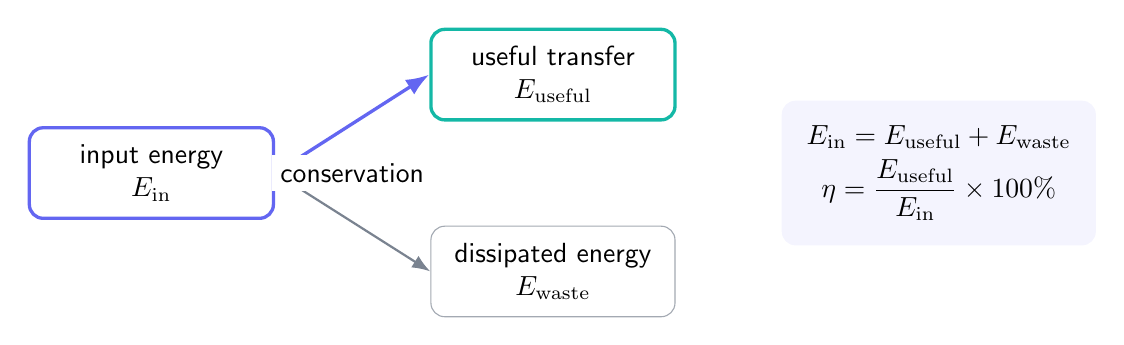
\begin{tikzpicture}[font=\sffamily,>=Latex,box/.style={draw=ink!45,rounded corners=5pt,minimum width=3.1cm,minimum height=1.15cm,align=center,fill=white}]
  \node[box,draw=nebula,very thick] (input) at (0,0) {input energy\\$E_{\rm in}$}; \node[box,draw=spark,very thick] (useful) at (5.1,1.25) {useful transfer\\$E_{\rm useful}$}; \node[box] (waste) at (5.1,-1.25) {dissipated energy\\$E_{\rm waste}$};
  \draw[->,very thick,nebula] (input.east)--(useful.west); \draw[->,thick,ink!65] (input.east)--(waste.west); \node[fill=white,inner sep=3pt] at (2.55,0) {conservation};
  \node[align=center,fill=nebula!7,rounded corners=5pt,inner sep=9pt] at (10.0,0) {$E_{\rm in}=E_{\rm useful}+E_{\rm waste}$\\[3pt]$\displaystyle \eta=\frac{E_{\rm useful}}{E_{\rm in}}\times100\%$};
\end{tikzpicture}
\end{document}
